\chapter{Integration of the compression unit
  in heat pumps layouts}
\label{chap:cp-intg}
\resetallacronyms

\begin{shaded}
  This chapter presents good practices and advanced proposals to
  integrate multistage oil-free variable-speed compression units in
  domestic heat pumps.
\end{shaded}

\section{Topology}
\label{sec:cp-intg-topology}

When using radial compressors, the vertical topology proposed with the
\BWP{} and presented in \cpref{fig:bwp-topology}, is advised. Indeed,
this vertical configuration makes the device more reliable and
increases the chances to collect liquid refrigerant where it is
functionally needed. Most companies building refrigeration circuits
with radial compressors use a vertical topology. The chillers produced
by Smardt\footnotep{Smardt (\url{http://www.smardt.com/}) is a company
  that makes chillers powered by Turbocor compressors. It has been
  created by one of the founders of the Turbocor company, after the
  latter was bought by Danfoss. Turbocor compressors
  (\url{http://www.turbocor.com/}) are radial compressors rotating on
  magnetic bearings. They typically power refrigeration applications
  above 50kW, as the magnetic bearings technology is not easy to scale
  down below this value.} are good examples of this design
rule. Additionally, using the vertical pipes leading to the
compression unit to protect it against the possible presence of
lubricant oil is a good practice. Those pipes can be sized following
the sizing rules presented by \citet{kesim-ileri-2000a} and
\citet{Guo-Shen-2011a}, in order to prevent that the oil is pulled up
with the gas stream.

\section{Electromagnetic perturbations}
\label{sec:cp-intg-electromag}

During the experiments performed with the \AWP{}, the signals of the
sensors where sometimes polluted with high levels of interferences
most probably caused by electro-magnetic perturbations, as the sensor
cables were not shielded. Those electro-magnetic perturbations were
probably generated by the three-phase inverter powering the motor of
the compression unit at high frequencies. Those interferences disturb
the calculation of essential values, like the superheat value. This is
clearly visible in \cpref{fig:awp-sh-too-low-ev-sh-with-plate}, where
the superheat calculation is perturbed (high frequency, high amplitude
signals) by the interferences on the pressure measurements, shown in
\cpref{fig:awp-electromagnetic-perturbation-P}. The temperature
measurements are not disturbed by interferences in that specific case
(as it can be seen in
\cpref{fig:awp-sh-too-low-ev-T-with-plate}). This example highlights
the importance to use shielded cables and grounded-sensors on this
type of device.

\section{Gas bearings aeration circuits}
\label{sec:cp-intg-aeration}

The lowest possible pressure level is favored in the gas bearings
cavity (component \#12) in order to minimize the gas bearings
losses. This implies that the outlet of the gas bearing aeration
circuit is connected to the zone of the heat pump circuit where the
pressure level is the lowest. The best location for this outlet is
consequently in the first stage separator. The inlet of the gas
bearings aeration circuit needs to be located in a zone with a higher
pressure level. Two solutions exist: the inlet can be either at the
intermediate pressure level, in the upper part of the economizer or
between the economizer and the second compression stage inlet, or
either at the higher pressure level, at the outlet of the second
compression stage. In the \BWP{} and the \AWP{}, the safest solution
has been favored: the gas bearings aeration circuit inlet is located
after the second compression stage outlet. This is the safest option,
since the expanded gas has a higher superheat value after its
expansion, if the gas comes from the second compression stage outlet,
and not from the economizer. With the pressure drop observed in the
\AWP{} aeration circuit, using the intermediate pressure level would
have resulted in a lower mass flow rate, which would have been too low
in the tested conditions. However, increasing the surface of the
0.5-\si{\micro\meter}-filter would certainly allow to take the
aeration flow from the economizer. Taking this flow at the economizer
would be better than taking it at the outlet of the second compression
stage, even if it is less safe. Indeed, the aeration flow, if removed
from the second compression stage flow rate, directly impacts the heat
pump efficiency, as the flow rate leaving the second compression stage
is used to provide the heating service. The level of superheat would
decrease a little, but this could be compensated with integration
strategies like the one exposed in
\cref{sec:next-topology}. Technically, it seems better to use the
intermediate pressure level to provide the aeration circuit with gas,
but economically, this needs to be studied further, as the filter
surface and volume would increase, in order to compensate for the
decrease of the pressure potential, in order to offer an equivalent
flow rate. This will most probably have an influence on the price of
the filter and consequently, on the price of the heat pump device.

\section{Towards new layouts with improved
  bypass circuits}
\label{sec:cp-intg-new-bypass}

The bypass circuits used in the \AWP{} were far from being
satisfactory, as detailed in \cpref{sec:awp-P-balance}. The bypass
circuit in the \BWP{} apparently performs better but was penalized by
the drawbacks highlighted in
\cpref{sec:bwp-bypass-mode-Pint-issue}. In order to solve this issue,
a new bypass principle is proposed, based on the bypass system of the
\BWP{}. This bypass system is presented in
\cref{fig:bwp-layout-maillefer-next-step,fig:awp-layout-next-step},
adapted to each tested prototype. This new concept mixes the
advantages observed with the economizer of the \AWP{}, which was in
two parts, and the compression stages in series of the \BWP{}. Indeed,
if the two parts of the economizer are connected with a check valve
that opens if liquid weights on it (the spring of the check valve must
be designed for this application, consequently), instead of a straight
pipe, the component \#27 of the \BWP{} becomes unnecessary. When
entering in bypass-mode, the solenoid valve above the pre-mixing
device\footnotep{On the left of the economizer in
  \cref{fig:bwp-layout-maillefer-next-step,fig:awp-layout-next-step},
  p.\,\pageref{fig:bwp-layout-maillefer-next-step}.}  shuts down the
arrival of liquid in the economizer (during this bypass-mode, the
second stage expansion valve must remain at least slightly open, in
order to prevent a possible pressurization of the pipe between the
expansion valve and the solenoid valve). The liquid in the economizer
leaves into the lower part of the economizer (if there is any in the
upper part). The two compressors are now in series. In this new
bypass-mode, either the heat pump cycle is used, either the bypass
circuit is used (in the contrary of the bypass circuit used in the
\BWP{}, which could be used in parallel of the heat pump circuit). If
the pressure level in the lower part of the economizer changes and
becomes higher than the pressure level in the upper part\footnotep{For
  instance, because some liquid evaporates, if there is any. The
  liquid could be used to cool down the power electronics, for
  instance, which would result in an evaporation of some of the
  fluid.}, the check valve opens and the pressure level are equal
again, which allows the check valve to close again. The pressure level
in the upper part of the economizer is consequently higher or equal to
the pressure level in the lower part. This bypass-mode can be used to
start and stop the cycle, in case of emergency, but also to evaporate
some liquid at the bottom of the first stage separator, as hot gas
returns to the first separator with a high superheat value. As
illustrated in
\cref{fig:bwp-layout-maillefer-next-step,fig:awp-layout-next-step},
the first separator can be equipped with a droplets
deflector\footnotep{A part designed to avoid the suction of droplets
  in the first compression stage.}, and the bypass circuit can deliver
the vapor directly at the bottom of the economizer. Blowing vapor
directly in the saturated liquid can result in the generation of
mist. The author's advice is to use metallic mesh or foam to trap the
droplets at the top of the deflector. This advice applies also to the
concept presented in \cref{sec:next-topology}. Bypass circuits need to
open if there is a power failure. Consequently, that part of the
circuit needs to be equipped with normally open valves.

\begin{figure}[htbp]
  \centering
  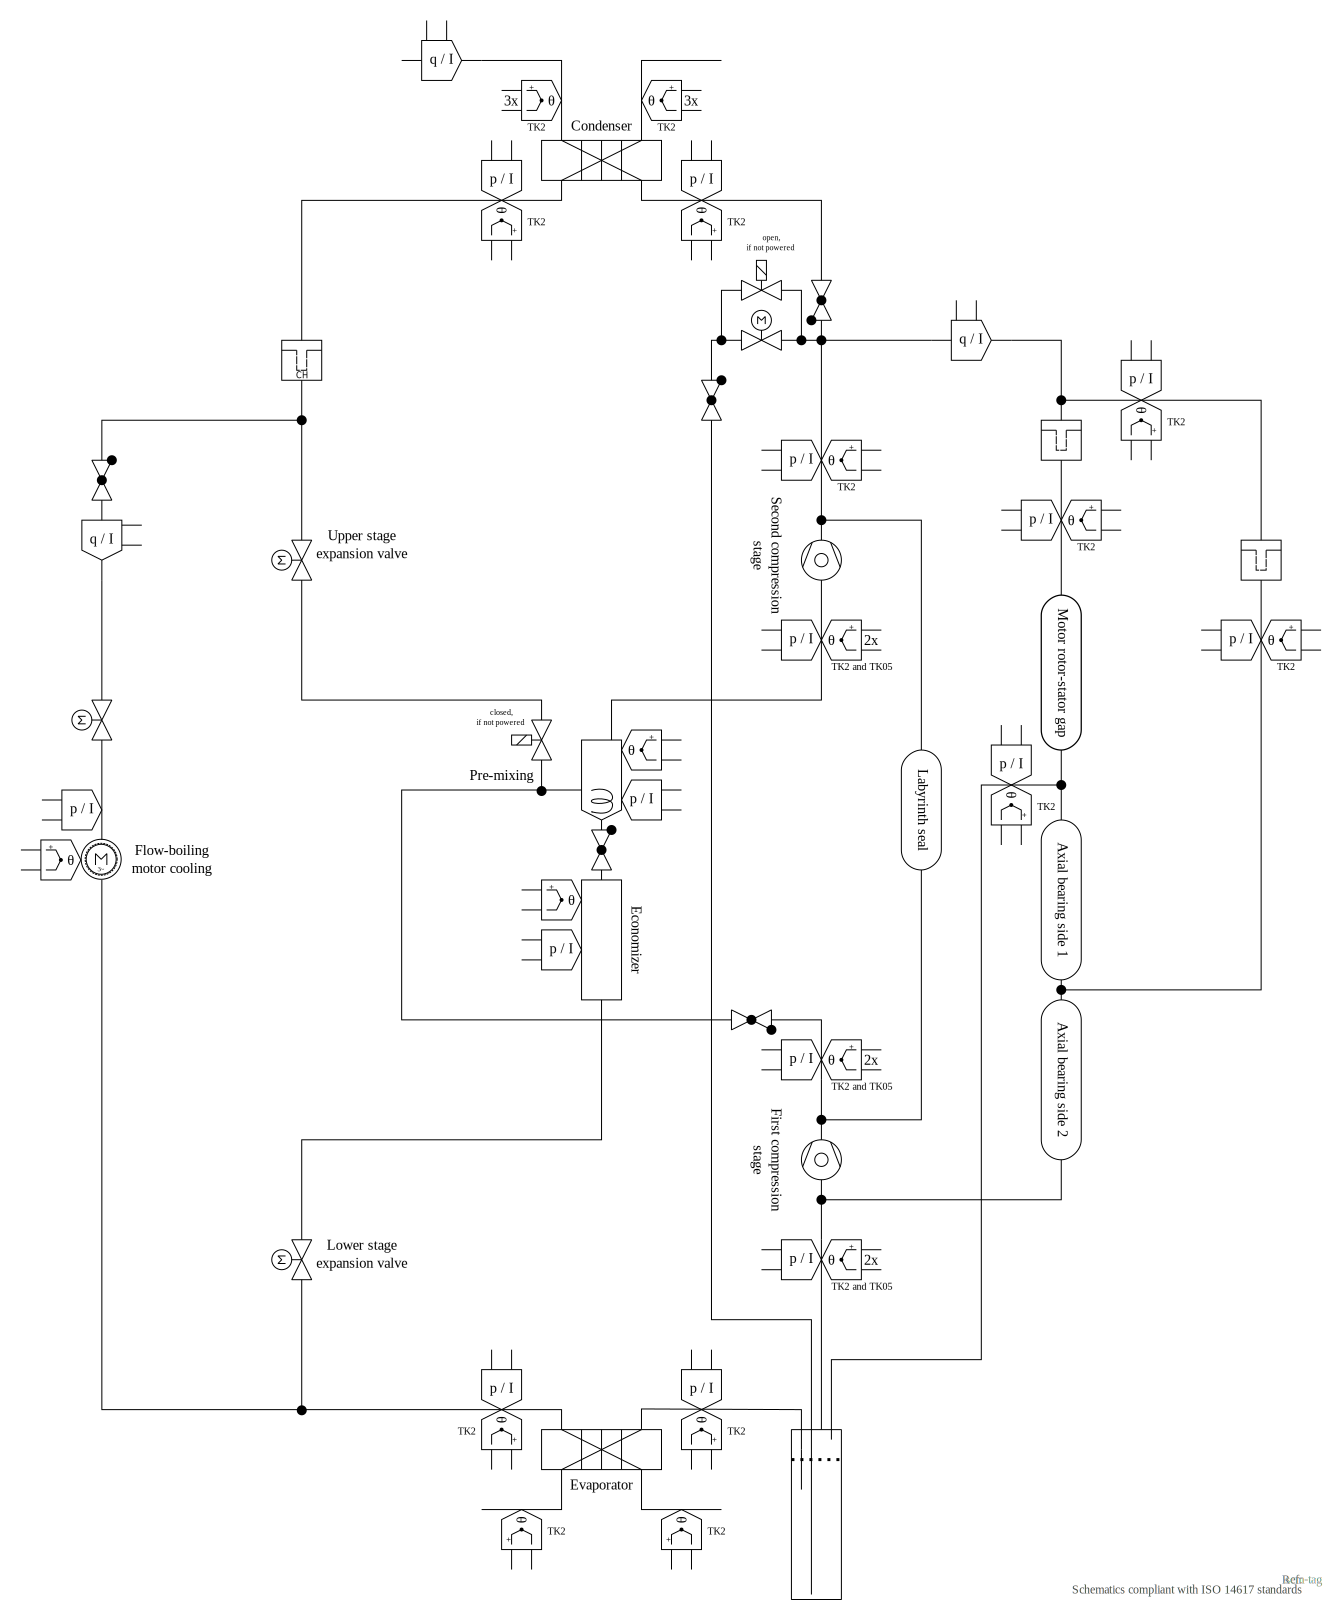
\includegraphics[width=\textwidth]{bwp-layout-maillefer-next-step}
  \caption[Proposal for a new BWP layout]
  {A new BWP layout}
  \label{fig:bwp-layout-maillefer-next-step}
\end{figure}

\begin{figure}[htbp]
  \centering
  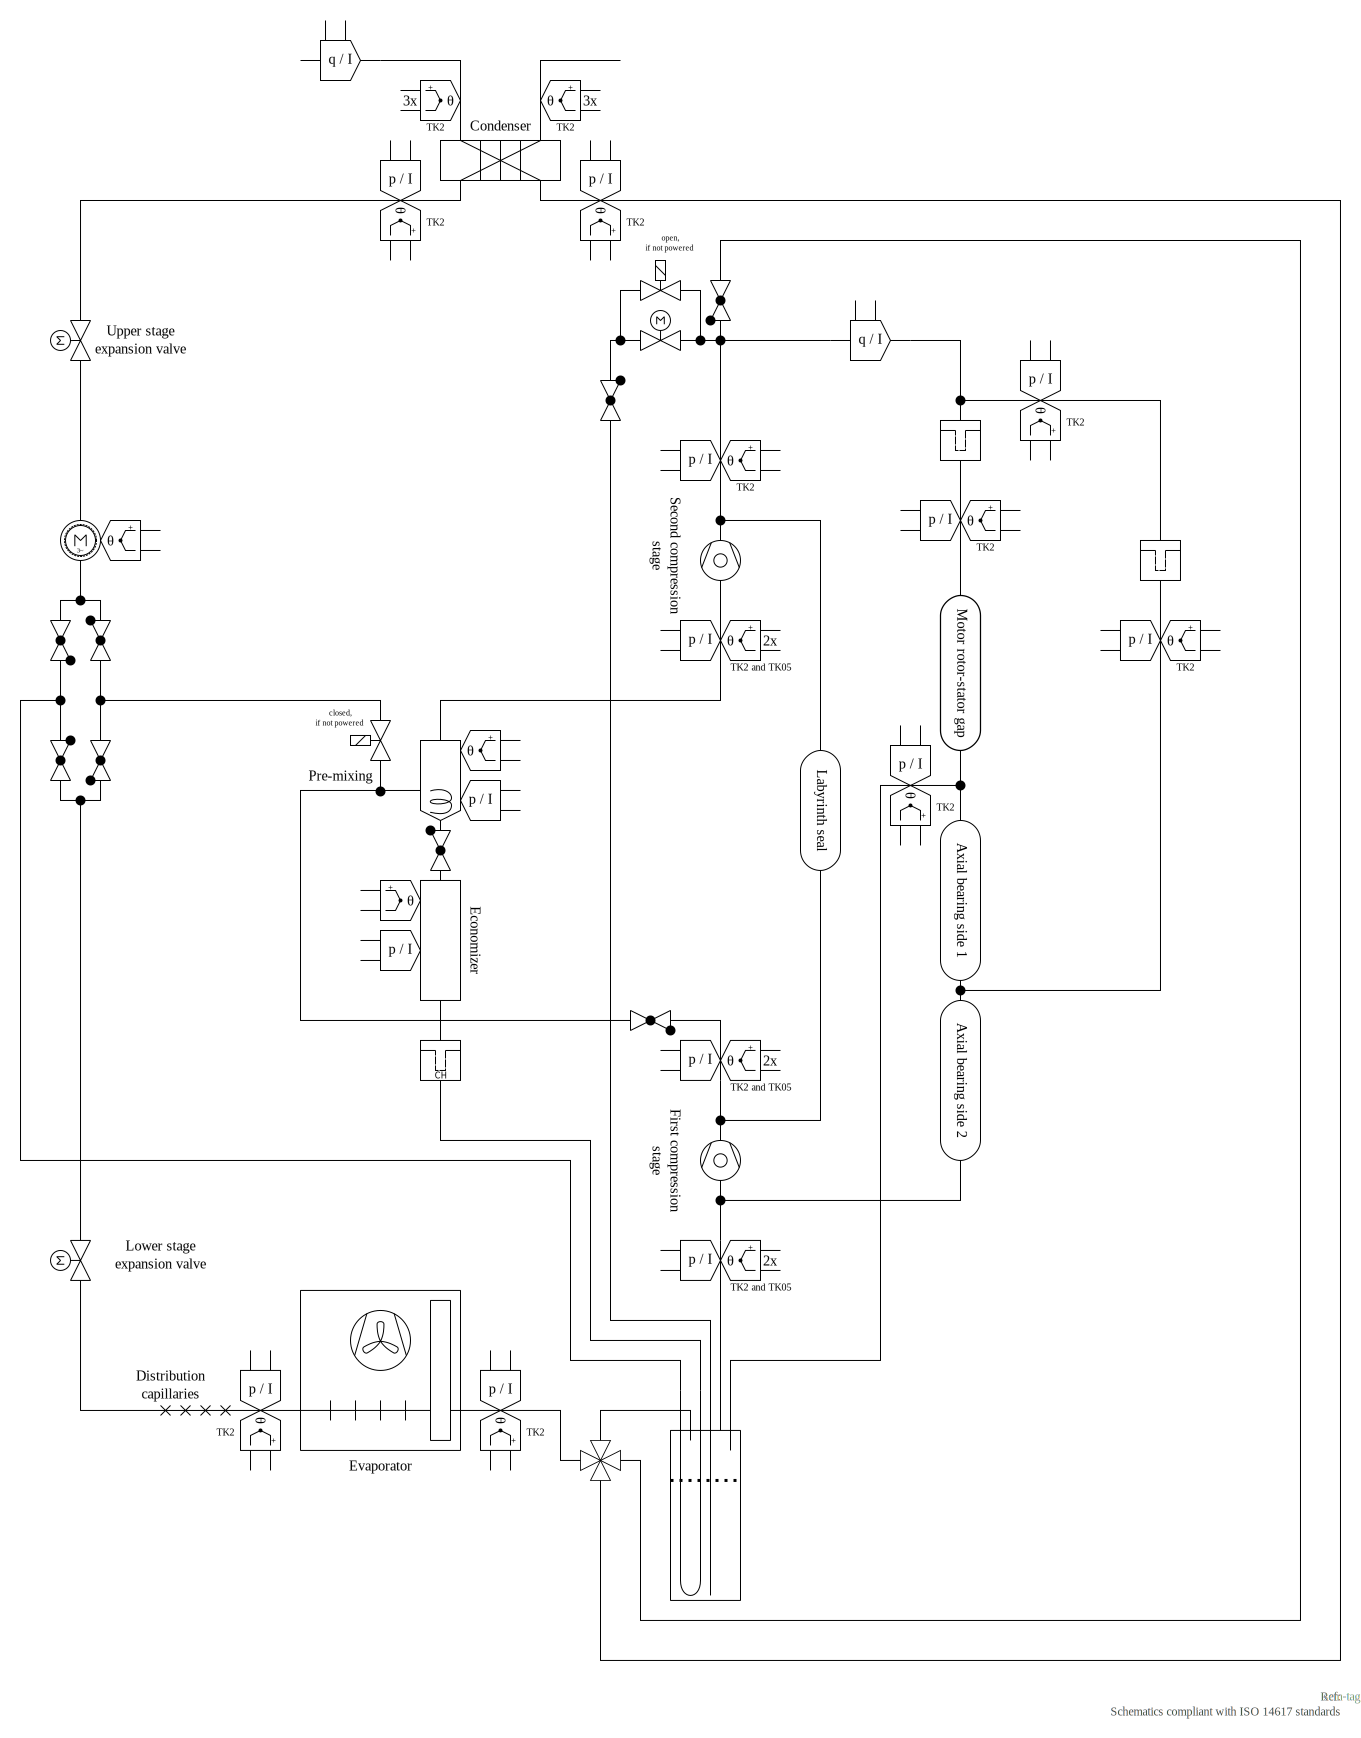
\includegraphics[width=\textwidth]{awp-layout-next-step}
  \caption[Proposal for a new AWP layout]
  {A new AWP layout}
  \label{fig:awp-layout-next-step}
\end{figure}

\section{Towards more integration, performance,
  and compactness}
\label{sec:next-topology}

The compression unit may allow a more advanced integration with the
heat pump cycle. This integration would lead to the creation of a
compression module containing many components of the heat pump
cycle. Indeed, the compression module can include easily the current
compression unit, the whole economizer, and the separator. In this
configuration, the only missing components to make a complete heat
pump cycle would be the condenser, the evaporator, the dryer-filter,
the two expansion valves, and the valves for the bypass and the gas
bearings aeration circuit. The module could even include the inverter,
cooled down by the liquid in the economizer. The inverter would be
located directly below the economizer, in that case, and would benefit
from passive convective cooling. As the inline components take almost
no volume, The volume of the installation is made from the volume of
the heat exchangers and of the compression unit module. As detailed in
\cpref{sec:sota-oilfree-hx}, the volume of the heat exchangers can be
decreased by taking advantage of the oil-free heat exchange
technologies. The compression module presented in
\cref{fig:next-prototype} is about 50cm-wide and 30cm-high. This
integration makes also the maintenance easier, as the technician can
unplug the module, and replace it easily. Functionally, such
integration brings many advantages:

\begin{figure}[h!tbp]
  \centering
  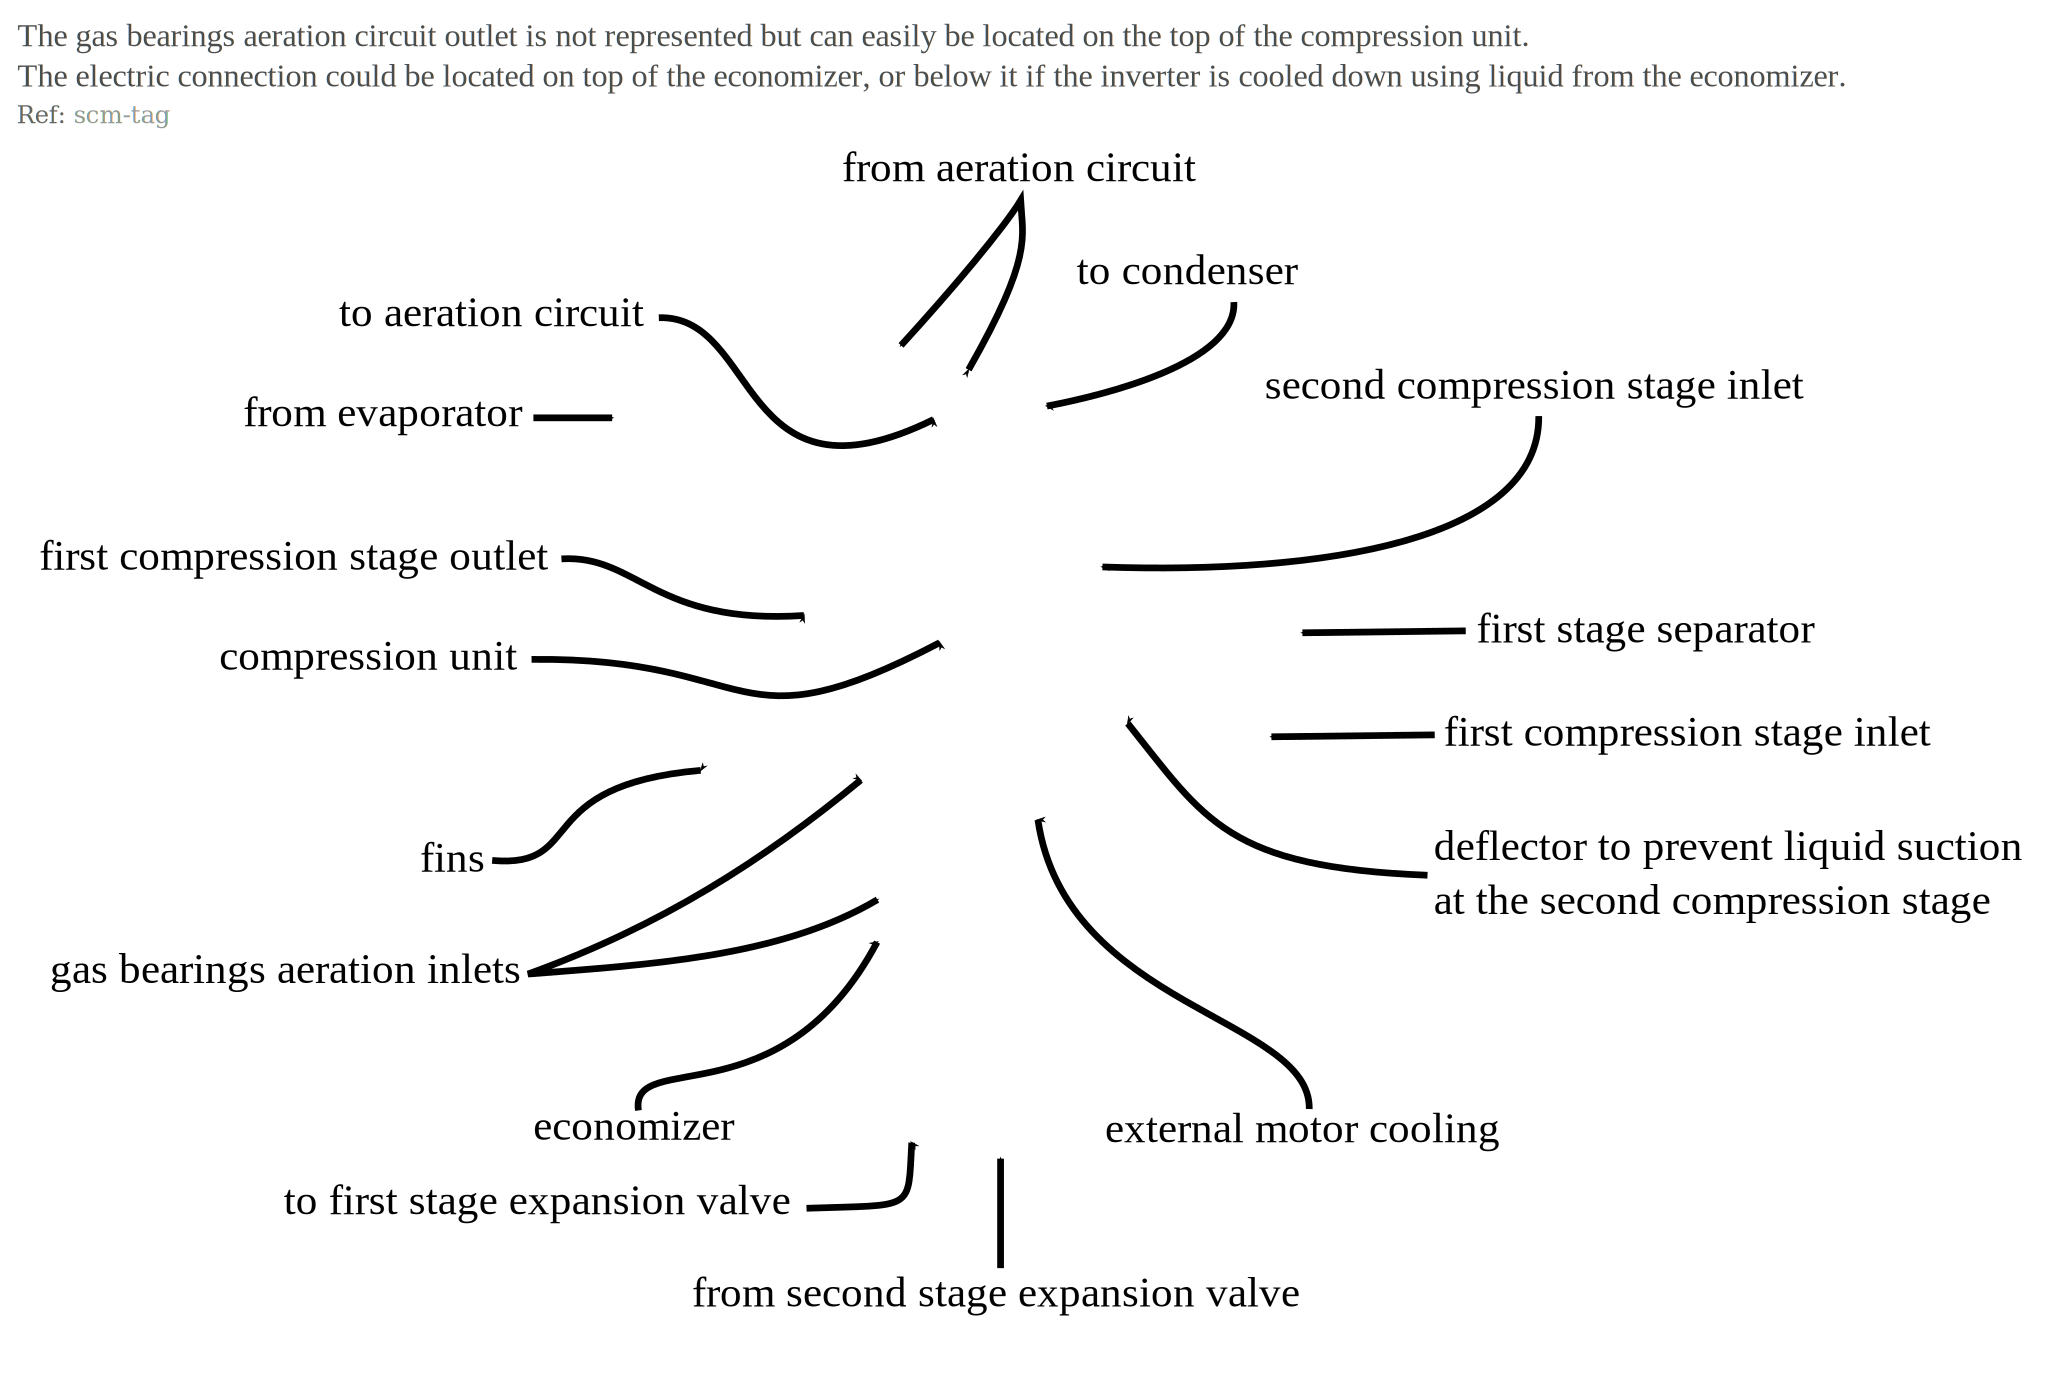
\includegraphics[width=\textwidth]{next-prototype}
  \caption{Proposal of an integrated topology for a future heat pump
    prototype}
  \label{fig:next-prototype}
\end{figure}

\begin{itemize}
\item There is no flow specifically taken to cool down the motor, so
  the heat pump controller is simpler. Moreover, the control itself is
  simpler, since the control of the heat pump depends on every flow
  rate in the cycle, as detailed in \cpref{sec:awp-issue-control}.
\item The check valves at the outlet of the compression stages can be
  integrated into the compression unit housing, like in scroll
  compressors.
\item The bypass system can be integrated into the compression unit
  housing, like in the turbo-compressors in cars.
\item The gas bearings aeration circuit is heated up by the liquid in
  the economizer. Indeed, the low pressure gas in the aeration circuit
  is colder than the liquid in the economizer. This protects the
  compression unit against the admission of droplets in the
  compression unit housing\footnotep{As the gas flow is limited in the
    gas bearings aeration circuits, condensation can occur, if the gas
    flow temperature is colder than the temperature around the pipe.}.
\item The gas from the evaporator would be heated up by the liquid in
  the economizer (the outside and the inside surfaces of the
  economizer can offer fins in order to increase the exchanges of heat
  energy), which protects the first compression stage against
  droplets. If droplets or liquid arrives in the first compression
  stage, it is evaporated by the heat transferred from the economizer.
\item With an effective deflector, the gas coming from the first
  compression stage can be blown directly in the saturated liquid in
  the economizer. This ensures that the gas which enters the second
  compression stage is at a saturated state. Moreover, as the distance
  between the economizer and the inlet of the second compression stage
  is almost equal to zero, there is almost no risk of condensation.
\item The flow coming from the second expansion valve, which is a
  two-phase flow, is ejected directly on the motor housing, which is
  equipped with fins, and the motor is effectively cooled down with a
  higher flow than in the current layouts, but with a stream at a
  higher temperature. This is a really good thing too, as condensation
  in the motor housing would be dangerous for the compression unit.
\end{itemize}

In order to secure the first tests, the author recommends the addition
of a joule heater around the compression unit housing, in order to
maintain the housing temperature above the condensation temperature in
every situation. The author thinks that this heater will be optional
in the final product, as strategies using the motor heat losses can be
applied before the real starting of the heat pump cycle. For instance,
when the installation is started, the cycle can stay in bypass-mode
with a low rotor speed\footnotep{For instance, a rotor speed of 60
  krpm would be appropriate.} until the temperature in the motor
housing and the bearings cavity is high enough. It would ensure that
no liquid is present in the compression unit before the real starting
up of the heat pump cycle.

\FloatBarrier
\bibliographystyle{plainnat}
\bibliography{main}
\label{sec:cp-intg-refs}
